\documentclass[10pt]{article}

\usepackage{amsfonts}
\usepackage{amsmath}
\usepackage{geometry}
\usepackage[dvipsnames]{xcolor}
\usepackage{graphicx}
\usepackage{subcaption}
\usepackage{listings}

\definecolor{codegreen}{rgb}{0,0.6,0}
\definecolor{codegray}{rgb}{0.5,0.5,0.5}
\definecolor{codepurple}{rgb}{0.58,0,0.82}
\definecolor{backcolour}{rgb}{0.95,0.95,0.92}
 
\lstdefinestyle{mystyle}{
    emph={init, RK, initialize},
    emphstyle=\color{PineGreen},
    commentstyle=\color{blue},
    keywordstyle={\color{BrickRed}\bfseries},
    numberstyle=\color{codegray},
    stringstyle=\color{codepurple},
    breakatwhitespace=false,         
    breaklines=true,                 
    captionpos=b,                    
    keepspaces=true,                 
    numbers=left,                    
    numbersep=5pt,                  
    showspaces=false,                
    showstringspaces=false,
    showtabs=false              
}

\title{Modeling Stars: \\ Two Method Comparison and Analysis}
\author{Najla Alahmadi, Michael Cock, Rebecca Halloran, Brady Metherall, Hector Robinson}

\newgeometry{margin=1in}
\setlength\parindent{0pt}

\begin{document}
\maketitle

\lstset{style=mystyle}

In this project, we modelled a spherically symmetric, static star by numerically integrating the four stellar equations. We started by doing this for a star that had the same core conditions as the sun, and then did many other stars. Using the results, we can find a relation between luminosity and temperature of the stars, and create an HR diagram. We were to create code that would be able to take a stars composition and mass to determine mainly temperature, luminosity and surface radius and build an HR diagram. Before we get there, lets talk about our program that will numerically integrate one star. \\

To perform the calculations we started from the core and integrated outward using the fourth order Runge-Kutta method. We specified a core pressure, core temperature, core density, and composition of the star. From there, the outward integration calculates total mass, luminosity, pressure, and temperature at every other radius. The integration stops when the boundary conditions are met, that is, the pressure goes to zero. Once this point is reached it means we are at the surface, we can take the temperature here, and use it for the HR diagram, Figure \ref{fig:code} shows samples of our code in greater detail. \\

\begin{figure}[htbp]
 \begin{subfigure}{\textwidth}
  \lstinputlisting[language=Python]{../solver/initialize.py}
  \caption{All constants are declared in \emph{initialize.py}.}
 \end{subfigure} \\
 \begin{subfigure}{\textwidth}
  \lstinputlisting[language=Python, firstnumber=7, firstline=7, lastline=17]{../solver/main.py}
  \lstinputlisting[language=Python, firstnumber=28, firstline=28, lastline=28]{../solver/main.py}
  \lstinputlisting[language=Python, firstnumber=56, firstline=56, lastline=56]{../solver/main.py}
  \caption{First \emph{main.py} calls \emph{initialize.init} to define our constants, then the core conditions are specified. We then open our data file, run our Runge-Kutta method, and then print the results to the data file.}
 \end{subfigure}
 \caption{Important sections of the code.}
 \label{fig:code}
\end{figure}

\begin{figure}[p]
\begin{centering}
 \begin{subfigure}{\textwidth}
  \input{./sunM}
 \end{subfigure} \\
 \begin{subfigure}{\textwidth}
  \input{./sunL}
 \end{subfigure} \\
  \begin{subfigure}{\textwidth}
  \input{./sunT}
 \end{subfigure} \\
   \begin{subfigure}{\textwidth}
  \input{./sunP}
 \end{subfigure}
 \caption{Simulation results of the Sun.}
 \label{fig:sun}
 \end{centering}
\end{figure}

Figure \ref{fig:sun} shows our results using the initial conditions of the core of the sun. These plots are as we would expect for a 1 solar mass star, but they do not get the exact values as expected. One thing that differs from our star to the sun is that it is only radiative for two radius steps, which is about $2\times 10^5$ meters, and convective for the rest. This is in contrast to the sun, where the radiative zone is about 70\% of the whole star. We were also unable to incorporate the optical depth so we used the surface temperature instead. The surface temperature should go to zero but our pressure hit zero first triggering the integration to stop. If we were able to use the temperature at a specific optical depth, we would have expected temperatures that produced a better HR diagram. We expect the final values for mass, luminosity, temperature, and pressure to be approximately $1 M_\odot$, $1 L_\odot$, $5770$ K, and $0$ Pa, respectively. \\

Knowing our model works properly but does not get proper values we can go further and get a general form of an HR diagram. By running this program for a total number of **number of stars** times we obtained the HR diagram shown in Figure \ref{fig:HR}. \\

We can see that is **looks similar to/does not really resemble** the known HR diagram. We can explore a well known program to get a sense of what the HR diagram should look like and compare it to our own model.  We will use MESA to do the comparison. This might not allow for a proper comparison because our model is static and has no rotation but it should give a general shape of the HR diagram. \\

\begin{figure}[p]
 \begin{centering}
  % GNUPLOT: LaTeX picture with Postscript
\begingroup
  \makeatletter
  \providecommand\color[2][]{%
    \GenericError{(gnuplot) \space\space\space\@spaces}{%
      Package color not loaded in conjunction with
      terminal option `colourtext'%
    }{See the gnuplot documentation for explanation.%
    }{Either use 'blacktext' in gnuplot or load the package
      color.sty in LaTeX.}%
    \renewcommand\color[2][]{}%
  }%
  \providecommand\includegraphics[2][]{%
    \GenericError{(gnuplot) \space\space\space\@spaces}{%
      Package graphicx or graphics not loaded%
    }{See the gnuplot documentation for explanation.%
    }{The gnuplot epslatex terminal needs graphicx.sty or graphics.sty.}%
    \renewcommand\includegraphics[2][]{}%
  }%
  \providecommand\rotatebox[2]{#2}%
  \@ifundefined{ifGPcolor}{%
    \newif\ifGPcolor
    \GPcolortrue
  }{}%
  \@ifundefined{ifGPblacktext}{%
    \newif\ifGPblacktext
    \GPblacktexttrue
  }{}%
  % define a \g@addto@macro without @ in the name:
  \let\gplgaddtomacro\g@addto@macro
  % define empty templates for all commands taking text:
  \gdef\gplbacktext{}%
  \gdef\gplfronttext{}%
  \makeatother
  \ifGPblacktext
    % no textcolor at all
    \def\colorrgb#1{}%
    \def\colorgray#1{}%
  \else
    % gray or color?
    \ifGPcolor
      \def\colorrgb#1{\color[rgb]{#1}}%
      \def\colorgray#1{\color[gray]{#1}}%
      \expandafter\def\csname LTw\endcsname{\color{white}}%
      \expandafter\def\csname LTb\endcsname{\color{black}}%
      \expandafter\def\csname LTa\endcsname{\color{black}}%
      \expandafter\def\csname LT0\endcsname{\color[rgb]{1,0,0}}%
      \expandafter\def\csname LT1\endcsname{\color[rgb]{0,1,0}}%
      \expandafter\def\csname LT2\endcsname{\color[rgb]{0,0,1}}%
      \expandafter\def\csname LT3\endcsname{\color[rgb]{1,0,1}}%
      \expandafter\def\csname LT4\endcsname{\color[rgb]{0,1,1}}%
      \expandafter\def\csname LT5\endcsname{\color[rgb]{1,1,0}}%
      \expandafter\def\csname LT6\endcsname{\color[rgb]{0,0,0}}%
      \expandafter\def\csname LT7\endcsname{\color[rgb]{1,0.3,0}}%
      \expandafter\def\csname LT8\endcsname{\color[rgb]{0.5,0.5,0.5}}%
    \else
      % gray
      \def\colorrgb#1{\color{black}}%
      \def\colorgray#1{\color[gray]{#1}}%
      \expandafter\def\csname LTw\endcsname{\color{white}}%
      \expandafter\def\csname LTb\endcsname{\color{black}}%
      \expandafter\def\csname LTa\endcsname{\color{black}}%
      \expandafter\def\csname LT0\endcsname{\color{black}}%
      \expandafter\def\csname LT1\endcsname{\color{black}}%
      \expandafter\def\csname LT2\endcsname{\color{black}}%
      \expandafter\def\csname LT3\endcsname{\color{black}}%
      \expandafter\def\csname LT4\endcsname{\color{black}}%
      \expandafter\def\csname LT5\endcsname{\color{black}}%
      \expandafter\def\csname LT6\endcsname{\color{black}}%
      \expandafter\def\csname LT7\endcsname{\color{black}}%
      \expandafter\def\csname LT8\endcsname{\color{black}}%
    \fi
  \fi
    \setlength{\unitlength}{0.0500bp}%
    \ifx\gptboxheight\undefined%
      \newlength{\gptboxheight}%
      \newlength{\gptboxwidth}%
      \newsavebox{\gptboxtext}%
    \fi%
    \setlength{\fboxrule}{0.5pt}%
    \setlength{\fboxsep}{1pt}%
\begin{picture}(8640.00,6480.00)%
    \gplgaddtomacro\gplbacktext{%
    }%
    \gplgaddtomacro\gplfronttext{%
      \csname LTb\endcsname%
      \put(176,4009){\rotatebox{-270}{\makebox(0,0){\strut{}$L$ ($L_\odot$)}}}%
      \put(4726,1254){\makebox(0,0){\strut{}$T$ (K)}}%
      \csname LTb\endcsname%
      \put(3871,1053){\makebox(0,0)[r]{\strut{}MESA star}}%
      \csname LTb\endcsname%
      \put(3871,833){\makebox(0,0)[r]{\strut{}MESA star}}%
      \csname LTb\endcsname%
      \put(3871,613){\makebox(0,0)[r]{\strut{}MESA star}}%
      \csname LTb\endcsname%
      \put(3871,393){\makebox(0,0)[r]{\strut{}MESA star}}%
      \csname LTb\endcsname%
      \put(3871,173){\makebox(0,0)[r]{\strut{}MESA star}}%
      \csname LTb\endcsname%
      \put(6706,1053){\makebox(0,0)[r]{\strut{}MESA star}}%
      \csname LTb\endcsname%
      \put(6706,833){\makebox(0,0)[r]{\strut{}MESA star}}%
      \csname LTb\endcsname%
      \put(6706,613){\makebox(0,0)[r]{\strut{}Real Stars}}%
      \csname LTb\endcsname%
      \put(6706,393){\makebox(0,0)[r]{\strut{}Simulated Stars}}%
      \csname LTb\endcsname%
      \put(1078,1804){\makebox(0,0)[r]{\strut{}$10^{-12}$}}%
      \csname LTb\endcsname%
      \put(1078,2245){\makebox(0,0)[r]{\strut{}$10^{-10}$}}%
      \csname LTb\endcsname%
      \put(1078,2686){\makebox(0,0)[r]{\strut{}$10^{-8}$}}%
      \csname LTb\endcsname%
      \put(1078,3127){\makebox(0,0)[r]{\strut{}$10^{-6}$}}%
      \csname LTb\endcsname%
      \put(1078,3568){\makebox(0,0)[r]{\strut{}$10^{-4}$}}%
      \csname LTb\endcsname%
      \put(1078,4010){\makebox(0,0)[r]{\strut{}$10^{-2}$}}%
      \csname LTb\endcsname%
      \put(1078,4451){\makebox(0,0)[r]{\strut{}$10^{0}$}}%
      \csname LTb\endcsname%
      \put(1078,4892){\makebox(0,0)[r]{\strut{}$10^{2}$}}%
      \csname LTb\endcsname%
      \put(1078,5333){\makebox(0,0)[r]{\strut{}$10^{4}$}}%
      \csname LTb\endcsname%
      \put(1078,5774){\makebox(0,0)[r]{\strut{}$10^{6}$}}%
      \csname LTb\endcsname%
      \put(1078,6215){\makebox(0,0)[r]{\strut{}$10^{8}$}}%
      \csname LTb\endcsname%
      \put(8243,1584){\makebox(0,0){\strut{}$10^{3}$}}%
      \csname LTb\endcsname%
      \put(4727,1584){\makebox(0,0){\strut{}$10^{4}$}}%
      \csname LTb\endcsname%
      \put(1210,1584){\makebox(0,0){\strut{}$10^{5}$}}%
    }%
    \gplbacktext
    \put(0,0){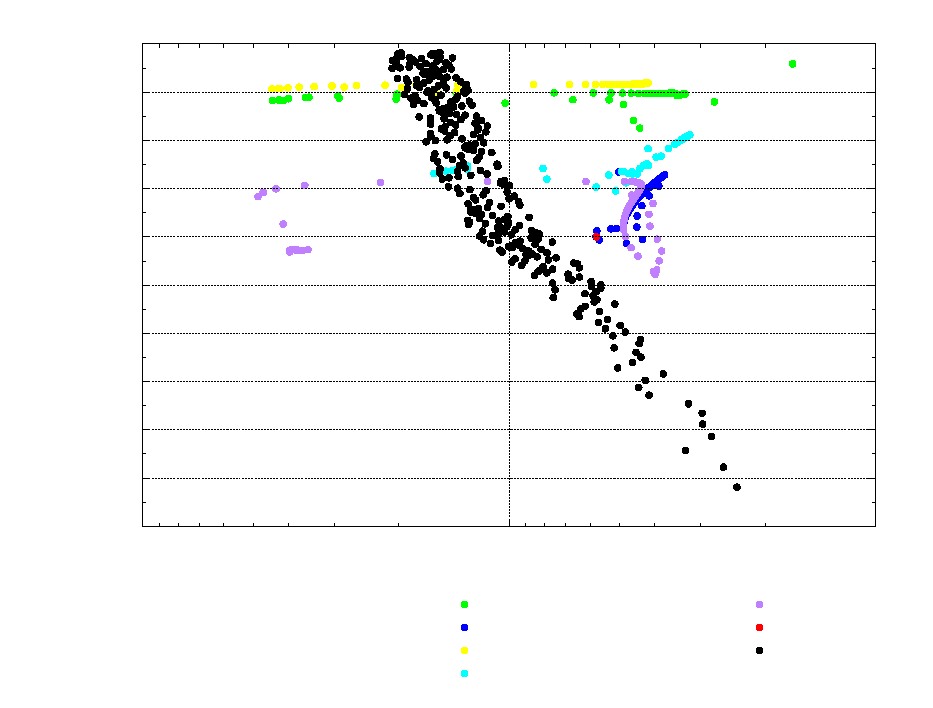
\includegraphics{./HR}}%
    \gplfronttext
  \end{picture}%
\endgroup

  \caption{Our reproduction of the HR diagram. The radius of the circles represents the radius of the s
tars.}
\label{fig:HR}
 \end{centering}
\end{figure}

\end{document}
